\documentclass{article}

\usepackage{amsmath}
\usepackage{amsfonts} % For math fonts.
\usepackage{amssymb} % For other math symbols not covered by amsmath.
\usepackage[pdftex]{graphicx} % For pictures, use \includegraphics[scale=decimal]{pic.png}; must be a .png file type.
\usepackage{multicol}
\usepackage{textcomp}
\usepackage[colorlinks = true, urlcolor = blue]{hyperref}
\usepackage{enumitem}
\usepackage{graphbox} 
\usepackage{subfig}
\usepackage{multicol}
\usepackage{nopageno}


\usepackage{tikz}
\usetikzlibrary{positioning, calc}
\usetikzlibrary{shapes.geometric,angles,quotes}
\usepackage{tikz-3dplot}


%page formatting
\usepackage{fullpage}
\setlength{\parindent}{0pt}


\newcommand{\tab}{\hspace*{0.25in}}
\newcommand{\csq}[1]{\reflectbox{''}#1''}  %This produces CS style quotes.
\newcommand{\csqt}[1]{\text{\reflectbox{''}#1''}}  %This produces CS style quotes as text.


\usepackage{listings}
\lstset
{ %Formatting for code in appendix
    language=Python,
    basicstyle=\footnotesize,
    numbers=left,
    stepnumber=1,
    showstringspaces=false,
    tabsize=2,
    breaklines=true,
    breakatwhitespace=false,
}


\begin{document}



%split_point

%\end{document}
Matt Priem \hfill Branching quiz\\
section 1\\
\begin{enumerate}
	\item 
		%https://edabit.com/challenge/8pDH2SRutPoaQghgc
		Luke Skywalker has friends and family, but he is getting older and having trouble 
		remembering them all.  Write a program that Luke (the user) can input a name and it 
		outputs the relation defined in the table below.
		\begin{center}
		\begin{tabular}{|l|l|} \hline
			Person 		& Relation \\ \hline \hline
			Darth Vader	& Father \\ \hline
			Leia		& Sister \\ \hline
			Han			& Brother in law\\ \hline
			R2D2		& Droid \\ \hline
		\end{tabular}\\ \hspace*{1in} *If he types any other name, report \csq{unknown}.
		\end{center}
		


	\item 
		Use the following code to answer the below questions\\
		\mbox{ \hspace*{0.25in}	\lstinputlisting[language=Python]{./code/c1.py}}
		\begin{enumerate}
			\item Find four values of my\_var so each of the four assignment statements will be executed: 
				each value should cause one assignment statement to be executed.
			\item Find four ranges of my\_var values that will cause each of the four assignment 
				statements to be executed.
		\end{enumerate}


	\item 
		Primary U.S. interstate highways are numbered 1-99.  Odd numbers (like 5 or 95) go north/
		south, and evens (like 10 or 82) go east/west.  Auxiliary highways are numbered 100-999, and 
		service the primary highway indicated by the rightmost two digits.  Thus, I-405 services 
		I-5, and I-290 services I-90.
		
		Note: 200 is not a valid auxiliary highway because 00 is not a valid primary highway 
		number.\\
		
		Let the user pick a highway number.  Given a valid highway number, indicate whether it runs 
		north/south or east/west.  If it is an invalid highway number, indicate that it is an 
		invalid highway number. \\
		For example,
		
		\hfill
		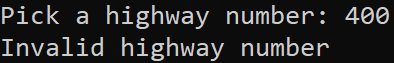
\includegraphics[width = 2in]{./imgs/highwayValidator1.PNG} \hfill
		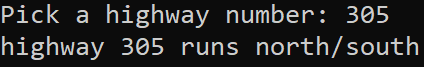
\includegraphics[width = 2in]{./imgs/highwayValidator2.PNG} \hfill \ 

		\hfill 
		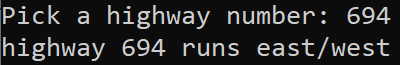
\includegraphics[width = 2in]{./imgs/highwayValidator3.PNG} \hfill 
		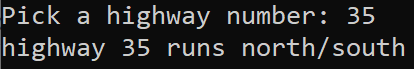
\includegraphics[width = 2in]{./imgs/highwayValidator4.PNG} \hfill \ 


\end{enumerate}
\pagebreak
Bart Simpson \hfill Branching quiz\\
section 1\\
\begin{enumerate}
	\item 
		%https://edabit.com/challenge/ancAxGEF9MsLWXDqe
		Write a program that asks the user for three side lengths of a triangle, and prints 
		the type of triangle.  The types of triangles are 
		\begin{itemize}
			\item No sides equal: \csq{scalene}
			\item Two sides equal: \csq{isosceles}
			\item All sides equal: \csq{equilateral}	
		\end{itemize}
		For example:

		\hfill 
		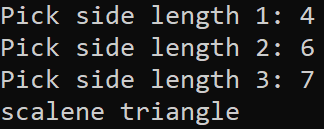
\includegraphics[height = 0.7in]{./imgs/typeOfTriangle1.PNG} \hfill 
		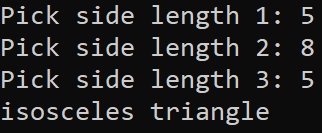
\includegraphics[height = 0.7in]{./imgs/typeOfTriangle2.PNG} \hfill  
		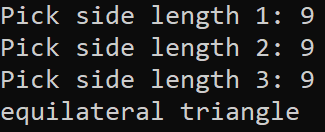
\includegraphics[height = 0.7in]{./imgs/typeOfTriangle3.PNG} \hfill \ 



	\item 
		Write a program that prompts the user to enter three integers and displays the integers 
		in decreasing order (largest to smallest).  You may not use the built-in functions 
		\textit{max}(), \textit{min}(), \textit{sort}() or \textit{sorted}().


	\item 
		(Game: heads or tails)  Write a program that lets the user guess whether the flip of a coin 
		results in heads or tails.  The program randomly generates an integer 0 or 1, which 
		represents head or tail.  The program prompts the user to enter a guess and reports whether 
		the guess is correct or incorrect.\\
		Hint: These should be your first two lines of code.
		\begin{verbatim}
		    from random import randint
		    value = randint(0,1) #picks a random integer. Either 0 or 1.
		\end{verbatim}



\end{enumerate}
\pagebreak
Lone Star \hfill Branching quiz\\
section 2\\
\begin{enumerate}
	\item 
		In your own words, describe the difference in logic of the following two sets of code:\\
		\begin{minipage}{.5\textwidth}
			(a) \mbox{\hspace*{2em} \lstinputlisting[language=Python]{./code/c2a.py}}
		\end{minipage}
		\begin{minipage}{.5\textwidth}
			(b) \mbox{\hspace*{2em} \lstinputlisting[language=Python]{./code/c2b.py}}
		\end{minipage}


	\item 
		%https://edabit.com/challenge/b8wRDMWgMZTN2nmfx
		Ask the user for three integers.  Determine (and output) how many copies of the same number 
		the user entered.\\
		For example, \\ \ \hfill
		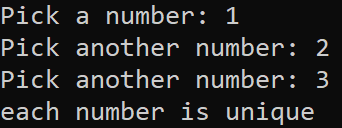
\includegraphics[height = 0.6in]{./imgs/uniqueIntCount1.PNG} \hfill
		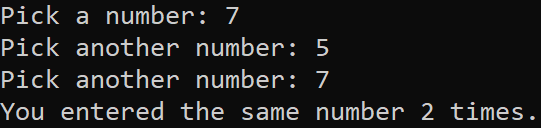
\includegraphics[height = 0.6in]{./imgs/uniqueIntCount2.PNG} \hfill \ 

	
	\item 
		The table below show what your resting heart rate should be based on age and athleticism.  
		Write a program that asks the user their age and desired athleticism goal, and then outputs 
		what their resting heart rate should be.

		\begin{minipage}{.45\textwidth}
			\begin{tabular}{c|cc}
				& \multicolumn{2}{c}{Athleticism}\\
				Age & Above Average & Below Average \\ \hline
				20 -- 39 & 47 -- 72 & 73 -- 93\\
				40 -- 59 & 46 -- 71 & 72 -- 94\\
				60 -- 79 & 45 -- 70 & 71 -- 97 \\
			\end{tabular}
		\end{minipage}
		\begin{minipage}{.45\textwidth}
			\vspace*{1em}
			Your end output should look similar to this
			\fbox{\parbox{\textwidth}{ Enter your age: 45\\
			Enter your athleticism goal: Below Average\\
			Your resting heart rate should be between 72--94.}}
		\end{minipage}


\end{enumerate}
\pagebreak
Dot Matrix \hfill Branching quiz\\
section 3\\
\begin{enumerate}
	\item 
		Primary U.S. interstate highways are numbered 1-99.  Odd numbers (like 5 or 95) go north/
		south, and evens (like 10 or 82) go east/west.  Auxiliary highways are numbered 100-999, and 
		service the primary highway indicated by the rightmost two digits.  Thus, I-405 services 
		I-5, and I-290 services I-90.
		
		Note: 200 is not a valid auxiliary highway because 00 is not a valid primary highway 
		number.\\
		
		Let the user pick a highway number.  Given a valid highway number, indicate whether it runs 
		north/south or east/west.  If it is an invalid highway number, indicate that it is an 
		invalid highway number. \\
		For example,
		
		\hfill
		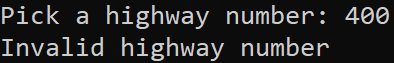
\includegraphics[width = 2in]{./imgs/highwayValidator1.PNG} \hfill
		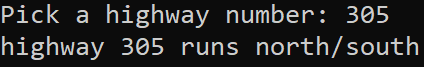
\includegraphics[width = 2in]{./imgs/highwayValidator2.PNG} \hfill \ 

		\hfill 
		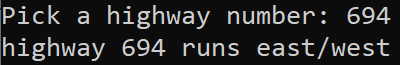
\includegraphics[width = 2in]{./imgs/highwayValidator3.PNG} \hfill 
		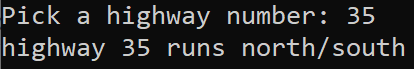
\includegraphics[width = 2in]{./imgs/highwayValidator4.PNG} \hfill \ 


	\item		
		The table below shows the maximum health of characters based on race and class for a new video game 
		I am creating.  Write a program that asks the user for the race and the class of their character, 
		and then sets the \textit{health\_points}	variable according to the table below.
		\begin{flushright}
		\begin{tabular}{c|cc}
			& \multicolumn{2}{c}{Race}\\
			Class & Elf & Ogre \\ \hline
			Warrior & 150 & 200\\
			Bard & 75 & 100\\
			Wizard & 25 & 50 \\
		\end{tabular}
		\end{flushright}
		
		\vspace*{-6em}
		\textit{health\_points} = -1\\
		\#Your code here.
		\vspace*{3em}		
		%\begin{tabular}{|ll}
		%	\\			
		%	\textit{health\_points} = -1 \\[5pt]
		%	\#Your code here. \\[5pt]
		%	& \\ & \\ & \\ & \\ & \\ & \\ & \\ & \\ & \\ & \\ & \\ & \\ & \\ & \\ & \\ & \\ & \\
		%	& \\ & \\ & \\ & \\ & \\ & \\ & \\ & \\ & \\ & \\
		%\end{tabular}


	\item 
		(Game: heads or tails)  Write a program that lets the user guess whether the flip of a coin 
		results in heads or tails.  The program randomly generates an integer 0 or 1, which 
		represents head or tail.  The program prompts the user to enter a guess and reports whether 
		the guess is correct or incorrect.\\
		Hint: These should be your first two lines of code.
		\begin{verbatim}
		    from random import randint
		    value = randint(0,1) #picks a random integer. Either 0 or 1.
		\end{verbatim}



\end{enumerate}
\pagebreak
Alfred Yankovic \hfill Branching quiz\\
section 2\\
\begin{enumerate}
	\item 
		Use the following code to answer the below questions\\
		\mbox{ \hspace*{0.25in}	\lstinputlisting[language=Python]{./code/c1.py}}
		\begin{enumerate}
			\item Find four values of my\_var so each of the four assignment statements will be executed: 
				each value should cause one assignment statement to be executed.
			\item Find four ranges of my\_var values that will cause each of the four assignment 
				statements to be executed.
		\end{enumerate}


	\item
		When driving in a car and approaching a traffic control light, \textit{green} means go, 
		\textit{yellow} means yield, and \textit{red} means stop.  Assuming there is a variable 
		named \textit{light\_color}, write a program that prints either the word \textit{go}, 
		\textit{yield}, or \textit{stop} depending of the value of \textit{light\_color}.  
		Let the user input the value of \textit{light\_color}.


	\item 
		(Game: heads or tails)  Write a program that lets the user guess whether the flip of a coin 
		results in heads or tails.  The program randomly generates an integer 0 or 1, which 
		represents head or tail.  The program prompts the user to enter a guess and reports whether 
		the guess is correct or incorrect.\\
		Hint: These should be your first two lines of code.
		\begin{verbatim}
		    from random import randint
		    value = randint(0,1) #picks a random integer. Either 0 or 1.
		\end{verbatim}



\end{enumerate}
\pagebreak
\end{document}